\chapter{Forward and Futures Markets}

These notes follow Robert J. Shiller's lecture on forward and futures markets, curated by LazyingArt LLC for the Yale lecture series. The lecture begins with a simple but far-reaching claim: futures markets matter because they give us prices for the future. From there the argument unfolds in a deliberate order. We begin with futures, forwards, and derivatives; we then pass through public hostility to speculation, the storage problem in grain, the historical invention of organized futures trading at Dojima, the modern agricultural term structure, the institutional logic of margin and daily settlement, the fair-value storage equation, the oil market and backwardation, and finally the extension to stock-index futures. The central idea is that a futures market is not merely a bet on tomorrow. It is an institution for organizing storage, standardizing commitments, and converting dispersed expectations into usable prices.

\section{Prices for the future}

A futures market is an organized market, much like a stock exchange, in which standardized contracts for future delivery are traded. A forward market is different. A forward contract is a bilateral arrangement between particular parties, with custom terms about grade, place of delivery, timing, remedies, and failure. Both are derivatives in the simple sense used in the lecture: their prices are derived from an underlying market.

The lecture insists on the larger point before the technical one. The future matters because planning matters. A household, a farm, a refinery, or a government must make decisions long before outcomes are realized, and futures markets place prices on those future contingencies. In that sense they are not merely side markets; they are among the economy's mechanisms for thinking ahead.

This is why the lecture pauses over the public dislike of derivatives. The word has become morally charged, especially after financial crises, but the lecture's claim is that the hostility is often directed at a misunderstood object. Derivatives require regulation, and the lecture says so explicitly, but there is nothing intrinsically sinister about them. On the contrary, they are part of the way a modern economy turns uncertain future conditions into present calculations.

That is the bridge to agriculture. If one wants to understand a futures market, one should begin where the economic function is transparent: grain must be stored, grain is seasonal, and grain prices necessarily connect today with later scarcity.

\section{Speculation, storage, and the grain market}

The lecture frames the issue with a survey question once asked in New York and Moscow: if grain traders hold grain in storage in anticipation of higher later prices, does that make shortages more common, or rarer? The striking result was that a majority of respondents, especially in New York, treated such speculation as socially harmful. The lecturer's point is that this reverses the elementary logic of storage.

There is usually one main harvest in the year. People do not consume the crop all at once. Therefore someone must carry inventories across time. Warehouses, traders, and grain merchants are not performing an accidental side activity; they are solving a fundamental intertemporal problem.

If those storage professionals believe that grain will be scarcer later, they hold more back now. That pushes the current price upward. The higher current price reduces current consumption and preserves inventories for later months. The result is not an arbitrary shortage created by greed. The result, in the lecturer's language, is a smoothing of supply over time.

\subsection{Question \& Answer}

\paragraph{Question.} Does speculation in grain create shortages, or can it help prevent them?

\paragraph{Answer.} In the logic of the lecture, it can help prevent them. If expected future scarcity raises the value of grain in storage, then grain is withheld now, the present price rises, present use falls, and more grain remains available for later delivery. The market is using a price increase today to reduce the severity of a shortage tomorrow. What appears morally suspect at first glance is, in this setting, the normal mechanism by which inventories are rationed over time.

This is the first economic mechanism of the chapter. The futures market does not create the storage problem. The storage problem already exists. The futures market makes the intertemporal calculation sharper, more visible, and more centralized.

\section{From Dojima to the standardized exchange}

The lecture then moves from economic function to institutional history. Futures trading, in the modern sense, begins in Japan, in Dojima, in Osaka. By 1673 there were dozens of rice warehouses there; the lecture cites a figure of $91$ warehouses. Rice was central to Japanese economic life, and Dojima served as a national rice market.

Before a true futures exchange existed, there were forward contracts. A rice merchant might arrange with a warehouse for regular future deliveries on custom terms. This is the natural beginning: forward contracts precede futures contracts. But forward markets carry two defects that matter enormously.

First, there is counterparty risk. If market conditions move against one side, that party may simply refuse to perform. If the price of rice falls, the merchant may disappear rather than take expensive contracted rice. If the price rises, the warehouse may try to escape a contract that now looks unfavorable.

Second, forward contracts are heterogeneous. One contract concerns one kind of rice, another insists on a particular delivery place, another has different quality conditions, another contains a special clause for defects or delay. Then one cannot even answer a seemingly simple question such as, ``What is the price of rice?'' There is no single clean object being priced.

The futures exchange solves both defects by standardization. Contracts specify a common commodity, a common delivery month, a common delivery location, and a common inspection regime. In the lecture's modern description, the exchange specifies the warehouse and the quality standards, and professional inspectors verify compliance. The contract may not be exactly what every trader wants, but it is now legible, tradable, and comparable.

The Dojima story also reveals that market design matters. Trading hours were enforced; a burning fuse reportedly marked the close; ``water men'' stopped traders who refused to stop; hand signals arose because the floor was too crowded and noisy for ordinary speech. These details are not merely colorful. They remind us that a futures market is an engineered institution.

\subsection{Question \& Answer}

\paragraph{Question.} What exact problem did the futures market solve that the forward market could not?

\paragraph{Answer.} It solved several related problems at once. It reduced bilateral counterparty risk, replaced idiosyncratic contract language with standardized terms, created a centralized and publicly interpretable price, and made contracts liquid enough to be traded rather than merely held to maturity. The lecture's historical point is that futures trading did not emerge because people wanted more abstraction. It emerged because bilateral custom contracting was too fragile and too opaque.

This is also why, in the lecture, the futures market ``almost becomes the real market.'' Farmers listening to price reports hear futures quotations, not some pure spot quotation, because the standardized futures price is often the clearest public price available.

\section{Agricultural futures, contango, and daily settlement}

The lecture turns next to modern agricultural futures, first rough rice and then wheat. The important caution is that a futures curve is a cross section at one date: prices today for delivery at different future maturities. It is not a time path of one contract. Once this is kept clear, the lecture introduces the most basic curve-shape vocabulary:

\begin{equation}
\text{contango: futures prices rise with maturity,}
\end{equation}

\begin{equation}
\text{backwardation: futures prices fall with maturity.}
\end{equation}

For rough rice, the lecture describes a pronounced upward slope. The front part of the curve rises from roughly $13.75$ to $15.5$ over about six months. As a simple numerical illustration, the gross increase is approximately
\begin{equation}
\frac{15.5-13.75}{13.75} \approx 0.127,
\end{equation}
or about $12.7\%$ over half a year. The lecturer uses this not as a claim of free expected return, but as the setup for a puzzle.

\subsection{Question \& Answer}

\paragraph{Question.} If the futures curve is steeply upward sloping, why is there not an easy riskless profit?

\paragraph{Answer.} The superficial trade is clear: buy grain now, store it, and sell futures against that inventory. But the trade is only ``riskless'' after we have paid for financing, warehousing, inspection, sanitation, insurance, and operational inconvenience. The lecture insists that professionals are already trying to exploit precisely these spreads. The existence of strong contango therefore attracts real storage effort rather than leaving a free gift unclaimed.

This observation leads to a broader point. A strong contango in grain is not merely a prediction. It is an incentive. It induces warehouse operators to search for additional storage capacity and to hold inventories over time. In the lecturer's framing, this is exactly how market self-interest can help prevent famine.

The lecture then returns to institutional structure. Futures exchanges largely remove counterparty risk by requiring margin and enforcing daily settlement. A trader can open a margin account, post something on the order of \$5{,}000, face a margin requirement on the order of $3\%$ to $5\%$, and thereby control perhaps \$100{,}000 of notional exposure. The price of the futures contract is not paid up front. Instead, the position is marked to market every day.

For a short futures position of size $Q$, the lecturer's verbal description can be written compactly as the note-writing reconstruction
\begin{equation}
M_{t+1}=M_t-Q\bigl(F_{t+1}-F_t\bigr),
\end{equation}
where $M_t$ is the margin balance and $F_t$ is the futures price on day $t$. If the futures price rises, the short loses and the margin account is debited. If the futures price falls, the short gains and the margin account is credited.

\subsection{Question \& Answer}

\paragraph{Question.} Why does daily settlement make a futures contract safer than a private forward contract?

\paragraph{Answer.} Because losses are realized continuously rather than postponed to the final delivery date. If adverse price movements deplete the posted margin, the broker asks for more collateral; if it is not supplied, the position is closed. The trader cannot simply disappear at maturity with a large unpaid loss. In the lecture's language, one is not really making a private contract with some unknown counterparty; both sides are making contracts with the exchange. That is why the resulting prices are much ``purer'' than forward prices burdened by bilateral default risk.

The wheat example reinforces the same logic. The front month is around \$7.23 per bushel, the curve is strongly upward sloping at short horizons, and then flattens or bends downward around the next harvest. The lecture's immediate interpretation is seasonal: contango compensates storage, but one should not expect inventories to be carried through harvest in the same way. Warehouses should be emptied and readied for the new crop.

\section{Fair value, storage cost, and convergence}

At this point the lecture introduces its main equation. The board presentation is important because the equation is written as a decomposition: one term for financing between now and maturity, one term for storage cost, and the label ``fair value'' underneath.

\begin{figure}[h]
\centering

\includegraphics[width=0.78\textwidth]{lecture_15_figure_02.png}
\caption{Blackboard fair-value equation for futures pricing.}
\end{figure}

The displayed relation is
\begin{equation}
P_F=(1+r+s)P_{\text{spot}}.
\end{equation}
Here $P_F$ is the futures price for a given maturity, $P_{\text{spot}}$ is the spot price today, $r$ is the total interest cost over the life of the contract, and $s$ is the storage cost over that same horizon. The lecture stresses that $r$ is not an annualized rate. If the annual interest rate is $5\%$, then for a one-year horizon we have
\begin{equation}
r=0.05,
\end{equation}
whereas for a horizon of one and a half years the corresponding total interest is about
\begin{equation}
r\approx 0.075.
\end{equation}

\paragraph{Worked derivation.} The lecture motivates the formula by thinking of futures markets as storage markets. One buys the commodity today, finances that purchase, stores the commodity until the delivery date, and at the same time sells a futures contract. In compact form:
\begin{align}
\text{cash outlay today} &= P_{\text{spot}},\\
\text{financing cost to maturity} &= rP_{\text{spot}},\\
\text{storage cost to maturity} &= sP_{\text{spot}},\\
\text{total carried cost} &= (1+r+s)P_{\text{spot}}.
\end{align}
If the futures price were materially above that carried cost, storage plus a short futures position would offer an excess profit opportunity. If it were materially below it, ordinary storage would be unattractive. Thus the lecture calls the relation a fair-value benchmark.

The lecture immediately adds a caution: the equation should not be treated as an exact literal identity. If it held with mechanical exactness, there would be no ordinary profit in storage. So the right way to read it is as a benchmark around which a working storage market must operate.

\subsection{Question \& Answer}

\paragraph{Question.} How can the futures price be above spot now and still end up equal to spot at expiration?

\paragraph{Answer.} Because the carry terms are horizon terms. As expiration approaches, there is less remaining time over which interest must be paid and less remaining time over which the commodity must be stored. Therefore the extra amount above spot shrinks as maturity approaches.

The lecture then reformulates the point dynamically. In a clean notation, its verbal convergence claim can be written as
\begin{equation}
T-t \downarrow 0
\quad \Rightarrow \quad
r(T-t),\, s(T-t)\downarrow 0
\quad \Rightarrow \quad
P_F(t,T)\to P_{\text{spot}}(T).
\end{equation}

The seasonal calendar-time sketch on the board is the lecture's way of slowing down this convergence argument and making it visual.

\begin{figure}[h]
\centering

\includegraphics[width=0.92\textwidth]{lecture_15_figure_03.png}
\caption{Fair-value formula beside the seasonal storage sketch.}
\end{figure}

In the perfect world described in the lecture, there is no harvest uncertainty. Wheat prices rise through the storage season because inventories are being carried, then collapse at harvest when new supply arrives, and then the cycle repeats. A fixed-maturity futures contract behaves differently. If the future harvest outcome were certain, then the futures price for a particular maturity date would simply equal the eventual spot price on that date; as calendar time passes, the spot price rises toward it and the carry wedge disappears.

\begin{figure}[h]
\centering
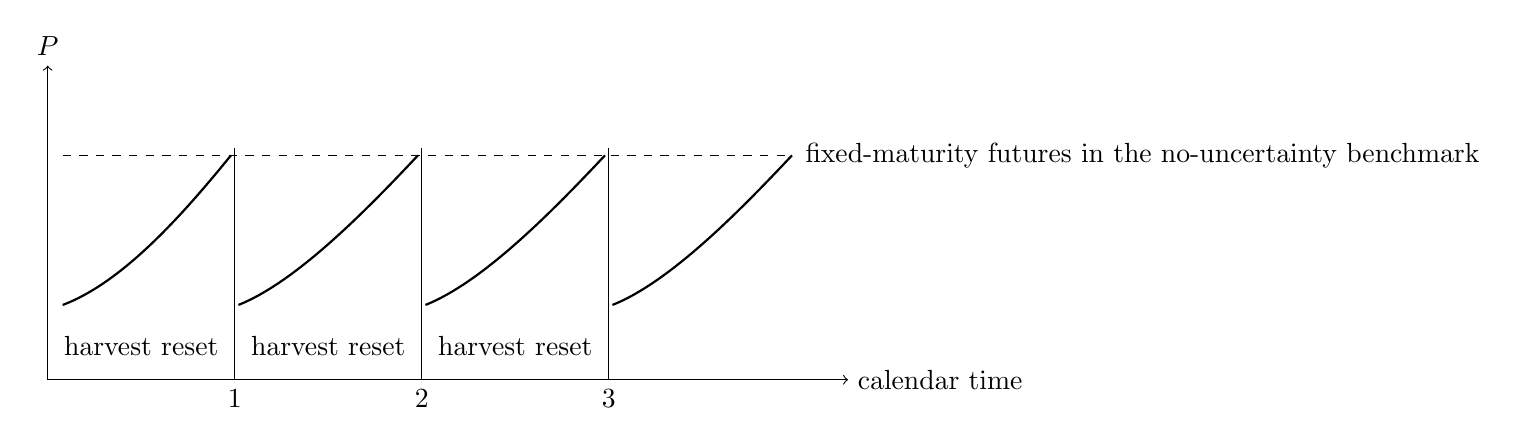
\begin{tikzpicture}[scale=0.95]
\draw[->] (0,0) -- (10.7,0) node[right] {calendar time};
\draw[->] (0,0) -- (0,4.2) node[above] {$P$};

\draw (2.5,0) -- (2.5,3.1);
\draw (5.0,0) -- (5.0,3.1);
\draw (7.5,0) -- (7.5,3.1);

\node[below] at (2.5,0) {$1$};
\node[below] at (5.0,0) {$2$};
\node[below] at (7.5,0) {$3$};

\draw[thick] (0.2,1.0) .. controls (1.0,1.3) and (1.8,2.2) .. (2.45,3.0);
\draw[thick] (2.55,1.0) .. controls (3.3,1.3) and (4.2,2.2) .. (4.95,3.0);
\draw[thick] (5.05,1.0) .. controls (5.8,1.3) and (6.7,2.2) .. (7.45,3.0);
\draw[thick] (7.55,1.0) .. controls (8.3,1.3) and (9.2,2.2) .. (9.95,3.0);

\draw[dashed] (0.2,3.0) -- (9.95,3.0);
\node[right] at (10.0,3.0) {fixed-maturity futures in the no-uncertainty benchmark};

\node at (1.25,0.45) {harvest reset};
\node at (3.75,0.45) {harvest reset};
\node at (6.25,0.45) {harvest reset};
\end{tikzpicture}
\caption{Stylized reconstruction of the lecture's calendar-time storage sketch. The curved segments represent within-year spot-price increases during storage; the dashed line represents the no-uncertainty benchmark for a fixed-maturity futures contract.}
\end{figure}

The lecture's verbal conclusion is now clear. Normally we expect contango. That is not because every commodity is destined to become scarce in a dramatic sense, but because carrying inventories forward in time has a cost.

\section{Oil, backwardation, and convenience yield}

The oil example is introduced precisely in order to create trouble for the simple formula. The projected crude-oil curve rises into late 2011, falls into early 2015, and then rises again farther out.

\begin{figure}[h]
\centering

\includegraphics[width=0.96\textwidth]{lecture_15_figure_04.png}
\caption{Board pricing relation next to the crude-oil futures curve.}
\end{figure}

The lecture emphasizes that the front-month crude-oil futures price is, in practice, the quoted ``price of oil.'' The true spot market is too heterogeneous and too thin to provide a single clean price. Oil is mostly sold through long-term contracts with many delivery and quality contingencies. The front month future is therefore the most public and legible price.

This is why the downward portion of the oil curve is such an instructive obstacle. If the front month is already very near spot because it is about to expire, and if the board equation says futures should exceed spot by financing and storage costs, how can a more distant contract lie below the present quoted price?

\subsection{Question \& Answer}

\paragraph{Question.} How can a futures curve slope downward if the fair-value formula adds interest and storage cost to spot?

\paragraph{Answer.} The lecture's answer is that the simple storage relation applies most naturally when the commodity is in storage as a carry trade. A downward-sloping curve indicates that no one plans to store the commodity for that span as an ordinary profit-seeking storage business. In such a case, the basic equation is no longer a complete description of the term structure.

The lecturer first states this heuristically: one may speak as if storage costs have become ``negative.'' The cleaner statement comes a moment later with the notion of convenience yield. A refinery or factory may continue holding oil even in backwardation because running its tanks to zero would be costly. The inventory itself provides a service: a buffer against disruption. That service has value.

The board later adds a faint note reading ``convenience yield,'' and the lecture's intended refinement may be written cautiously as
\begin{equation}
P_F \approx (1+r+s-y)P_{\text{spot}},
\end{equation}
where $y$ is a convenience yield. This is a lecture-aligned reconstruction rather than a verbatim board transcription, but it captures the logic of the discussion. A sufficiently large convenience yield can offset financing and storage costs and permit backwardation.

\begin{figure}[h]
\centering

\includegraphics[width=0.92\textwidth]{lecture_15_figure_05.png}
\caption{Fair-value equation revisited with convenience-yield discussion.}
\end{figure}

The lecture's careful caveat should be preserved. The simple storage formula is most trustworthy when the commodity is genuinely being carried in storage. It need not describe every point on every futures curve once storage incentives weaken or once inventory has a direct operational value that ordinary carrying-cost language does not fully express.

\section{Oil history and financial futures}

After resolving the local puzzle, the lecture widens the frame. Oil matters on a civilizational scale. The world price history of oil, running from the nineteenth century to the present, is invoked to show how unusual the stable middle decades were and how disruptive the later shocks became.

The lecture's rough chronology is this. Early oil prices moved with discoveries and new uses. Later, especially during the era of the Texas Railroad Commission, prices were relatively stable. Then the first oil crisis of 1973--74 broke that stability and helped prompt the development of oil futures. The second oil crisis of 1979--80 reinforced the importance of organized futures trading. Later spikes, including the 2008 surge above \$140 per barrel, again showed how energy shocks can feed into major recessions.

The lecture's institutional point is the same as before, but the stakes are larger. Oil futures are not peripheral casino objects. They are instruments through which producers, refiners, and users manage one of the largest and most consequential price risks in the world economy. The total value of oil in the ground is enormous, and extraction decisions are made against the background of futures prices.

The final move is to financial futures, especially the S\&P 500 index futures market. The contractual form changes: delivery is by cash settlement rather than by trucks arriving at a warehouse. But the fair-value logic survives.

Stocks do not impose a physical storage cost. Instead they pay dividends. In the lecture's language, storage cost is effectively negative. With cleaned notation, the stock-index version of fair value is therefore
\begin{equation}
P_F \approx (1+r-y)P_{\text{spot}},
\end{equation}
where now $y$ denotes the dividend yield over the relevant horizon. The transcript is slightly garbled at this point, so this equation should be read as a careful reconstruction of the intended structure, not as a literal transcript of every spoken symbol.

The qualitative implication is straightforward. Whether stock-index futures lie above or below spot depends on the balance between financing cost and dividend yield. The lecture notes that, at the time of speaking, short interest rates were near zero while dividend yields were around $2\%$, so short-horizon stock-index futures could naturally trade below spot. At longer horizons the balance might reverse.

This is the lecture's final contrast. Some futures curves, such as those for oil or grain, can be genuinely informative about scarcity, storage, and inventory conditions. Others, such as stock-index futures and often gold futures, are largely carrying-cost relations. They are much less informative about the future path of the underlying price than a casual observer might imagine.

\section{Summary}

The lecture begins with a philosophical point and ends with a technical distinction, but the through-line is continuous. Futures markets give us prices for the future. They become socially valuable because storage, planning, and risk-bearing all require such prices.

Agricultural examples make the mechanism visible. Grain must be stored; contango compensates storage; speculation can smooth scarcity; and the organized futures exchange improves on bilateral forward contracting by standardizing terms and removing most counterparty risk through margin and daily settlement.

The carrying-cost benchmark
\[
P_F=(1+r+s)P_{\text{spot}}
\]
then provides the chapter's mathematical center. It explains why futures often exceed spot and why convergence occurs at expiration. Oil shows the limit of the simplest version of that formula and forces the refinement through convenience yield. Financial futures show a cleaner case: when the underlying is always ``in storage,'' the futures curve may reveal little more than fair value itself.

The result is a coherent picture. Futures markets are institutions in which history, storage, regulation, and mathematics meet.